% PAKETE UND DOKUMENTKONFIGURATION
\documentclass[11pt, a4paper]{article}

% Encoding für Umlaute
\usepackage[utf8]{inputenc}
\usepackage[T1]{fontenc}

% Silbentrennung
\usepackage[ngerman]{babel}

% erweiterte Matheumgebungen und Formelnummer mit Sectionnummer
\usepackage{amsmath}
\numberwithin{equation}{section}

% Braket Notation
\usepackage{braket}
\usepackage{isotope}
\usepackage[version=4]{mhchem}
\usepackage{tensor}
\usepackage{slashed}

% zusätzliche mathematische Schriftarten
\usepackage{amsfonts}

% verschiedene mathematische Symbole
\usepackage{amssymb}

% sidewaysfrac
\usepackage{xfrac}

% Einheiten setzen z.B. \SI{10}{\kilo\gram\meter\per\second\squared}
% Fehler: \SI{10 +- 0,2e-4}{\metre}
\usepackage{siunitx}
\sisetup{
  output-decimal-marker={,},
  separate-uncertainty
}

% Einheitendefinitionen
\DeclareSIUnit{\skt}{Skt.}
\DeclareSIUnit{\gauss}{G}
\DeclareSIUnit{\division}{div.}
\DeclareSIUnit{\Kanal}{Kanal}

% Operatordefinitionen
\DeclareMathOperator{\erf}{erf}

% Randbreiten
\usepackage[left=3.5cm,right=3.5cm,top=3cm,bottom=3cm,twoside]{geometry}

% Bilder einfügen
\usepackage{graphicx}
\usepackage[percent]{overpic}

% Textfarbe
\usepackage{color}

% Verweise innerhalb des Dokuments
\usepackage{hyperref}
\hypersetup{
	colorlinks = true,
	allcolors = {black}
}

% bessere Tabellenlayouts
\usepackage{booktabs}
\usepackage{multirow}
\usepackage{multicol}

% Seitenlayout (Kopfzeile)
\usepackage{fancyhdr}

% Float Barriers
\usepackage{placeins}

% Pakete für gedrehte Subfigures
\usepackage{caption}
\usepackage{subcaption}
\usepackage{rotating}
\usepackage{capt-of}

% Paket für textumflossene Abbildungen und Tabellen
\usepackage{wrapfig}

\usepackage{float}

% Caption-Setup
\captionsetup{font={small}}
\renewcommand{\thefigure}{\thesection.\arabic{figure}}
\renewcommand{\thesubfigure}{\alph{subfigure}}
\renewcommand{\thetable}{\thesection.\arabic{table}}
\renewcommand{\thesubtable}{\alph{subtable}}

% Manuelle Silbentrennung
\hyphenation{Sekundär-elek-tronen-verviel-facher}

% Tiefe des Inhaltsverzeichnisses (Level: 1 sections, 2 subsections,
% 3 subsubsections)
\setcounter{tocdepth}{3}

% FANCYHDR SETUP
\pagestyle{fancy}
\fancyhead[EL,OR]{\thepage}
\fancyhead[ER]{\leftmark}
\fancyhead[OL]{\rightmark}
\setlength{\headheight}{13.6pt}

\renewcommand{\sectionmark}[1]{
\markboth{\thesection{} #1}{\thesection{} #1}
}
\renewcommand{\subsectionmark}[1]{
\markright{\thesubsection{} #1}
}

\newcommand{\korr}[1]{{\color{red}(#1)}}

% DOKUMENTINFORMATIONEN
\title{A248 \\ Magneto-optische Falle}

\author{Christopher Deutsch\footnote{christopher.deutsch@uni-bonn.de} \and Christian Bespin\footnote{christian.bespin@uni-bonn.de}}

\date{\today}

\begin{document}

\begin{titlepage}

\maketitle

% DURCHFÜHRUNGSDATUM UND TUTOR
\begin{center}
\begin{tabular}{l r}
Durchführung: & 4./5. April 2016 \\
Gruppe: & P8 \\
Tutor: & Daniel Babik
\end{tabular}
\end{center}

% ZUSAMMENFASSUNG
\begin{abstract}
\noindent
\end{abstract}

\end{titlepage}

% INHALTSVERZEICHNIS
\tableofcontents
% Neue Seite nach TOC
\newpage

% INHALT VERSUCHSPROTOKOLL
\section{Einführung}

Das Ziel von Atomfallen ist die Speicherung von Atomen in einem festgelegten Raum.
Um dies zu ermöglichen müssen sich die Atome kaum bewegen, so dass diese zunächst gekühlt und anschließend durch geeignete Mechanismen daran gehindert werden müssen, sich frei im Raum zu bewegen.
Ein solcher Aufbau kann durch eine sogenannte magneto-optische Falle realisiert werden, die in diesem Praktikumsversuch in Betrieb genommen und charakterisiert werden soll.

\section{Theorie}

\korr{Hier noch kurze Einführung}

\begin{figure}
	\centering
	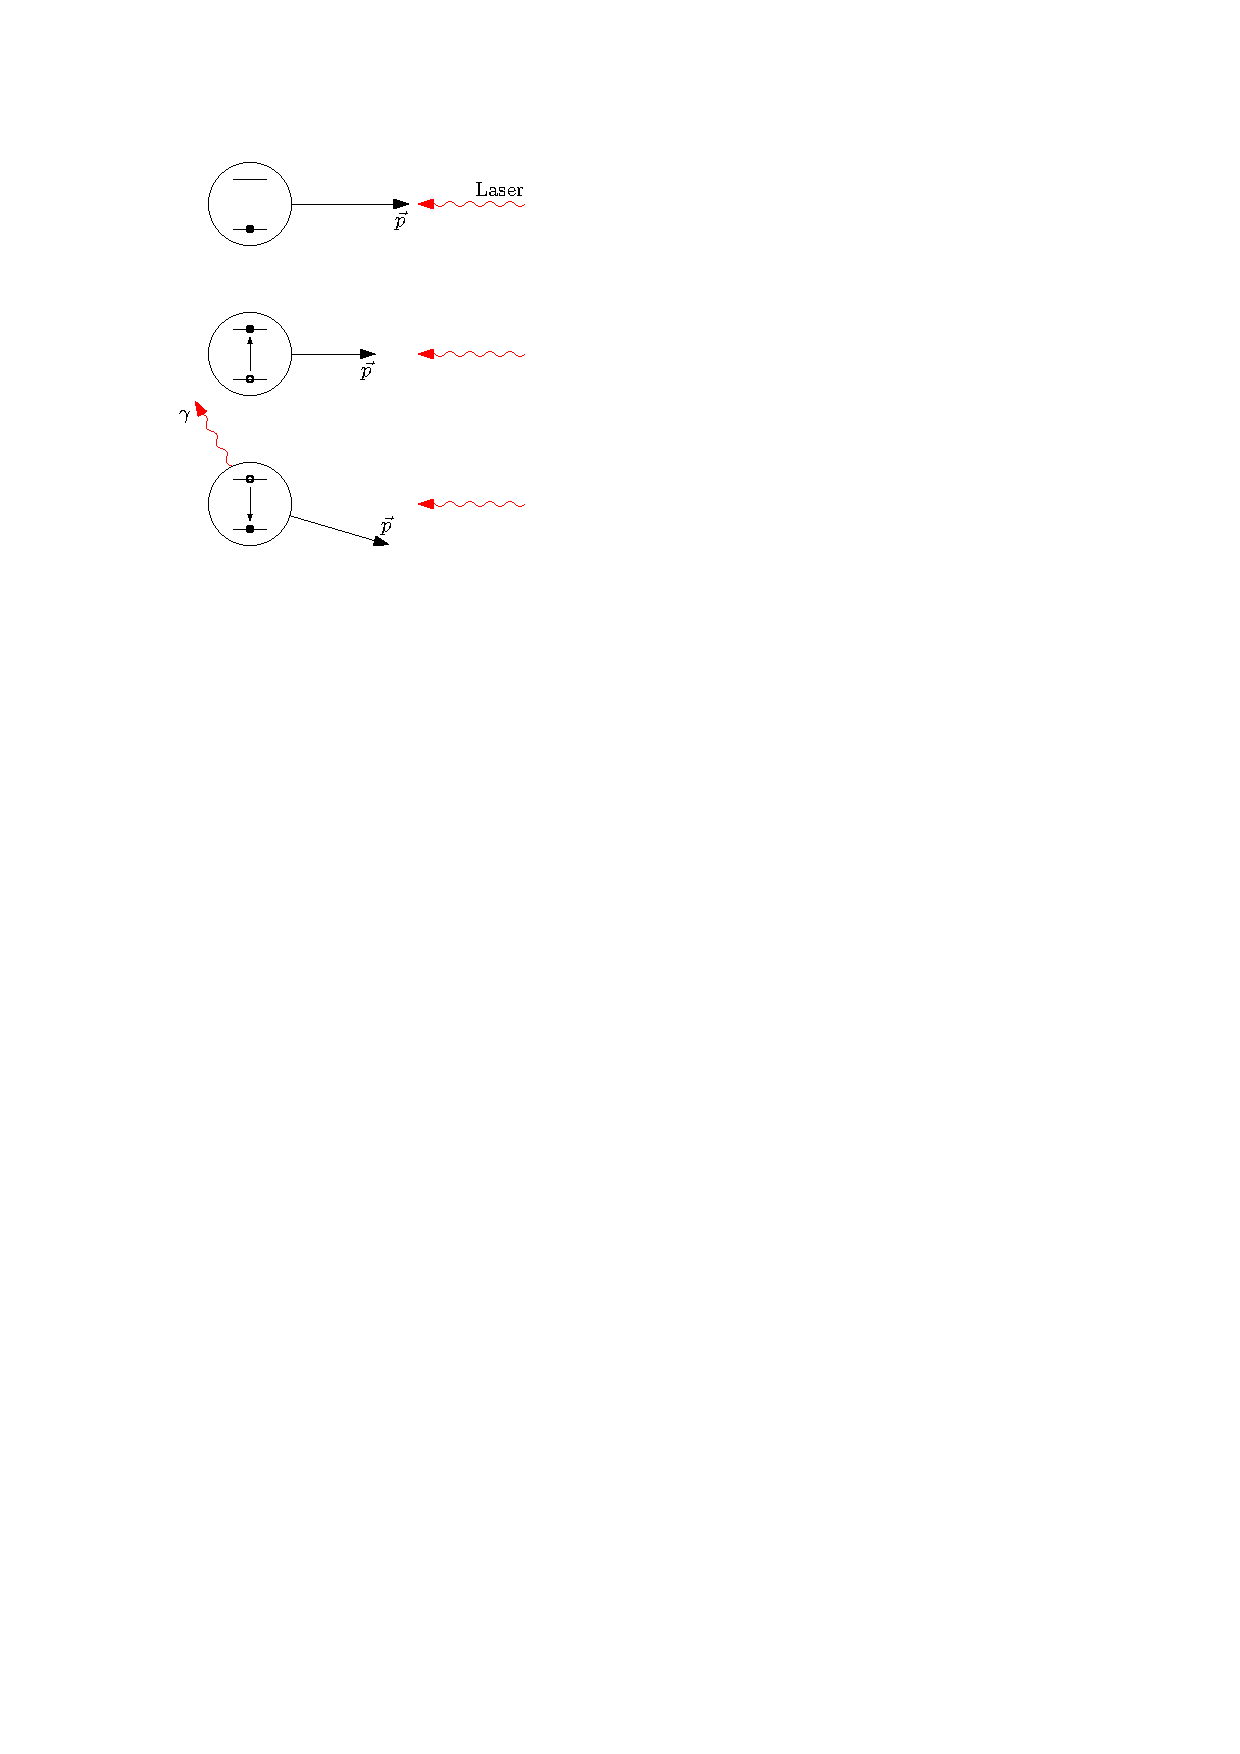
\includegraphics{./figures/theory/streukraft.pdf}
	\caption{Streukraft}
\end{figure}

\subsection{Laserkühlung}

Zum Kühlen der Atome wird Laserlicht genutzt, das entgegen der Flugrichtung der Atome eingestrahlt wird.
Der Impuls eines Photons $\hbar k$ mit der Wellenzahl $k$ kann das Atom mit der Übergangsenergie $\hbar\omega = \hbar c k$ resonant anregen, wobei die Richtung des bei der Abregung entstehenden Photons zufällig ist.
Für eine Vielzahl einfallender Photonen ist die Emission dann isotrop und es resultiert ein Impulsübertrag auf das Atom, welcher dieses bremst.
Da sich das Atom jedoch bewegen kann und wegen seiner Geschwindigkeit $v$ das Laserlicht aufgrund des Dopplereffekts mit einer um $kv$ verschobenen Frequenz als der im Laborsystem wahrnimmt, wird der Laser rotverstimmt, d.h. mit einer geringeren Frequenz als für den atomaren Übergang nötig, betrieben.
Aufgrund des Dopplereffekts nimmt ein Atom, welches sich also entgegen der Richtung des Laserstrahls bewegt, das Licht des Laser mit einer Frequenz wahr, welche das Atom in den angeregten Zustand versetzt und es aufgrund der isotropen Emission kühlt.
\begin{figure}[h]
	\centering
	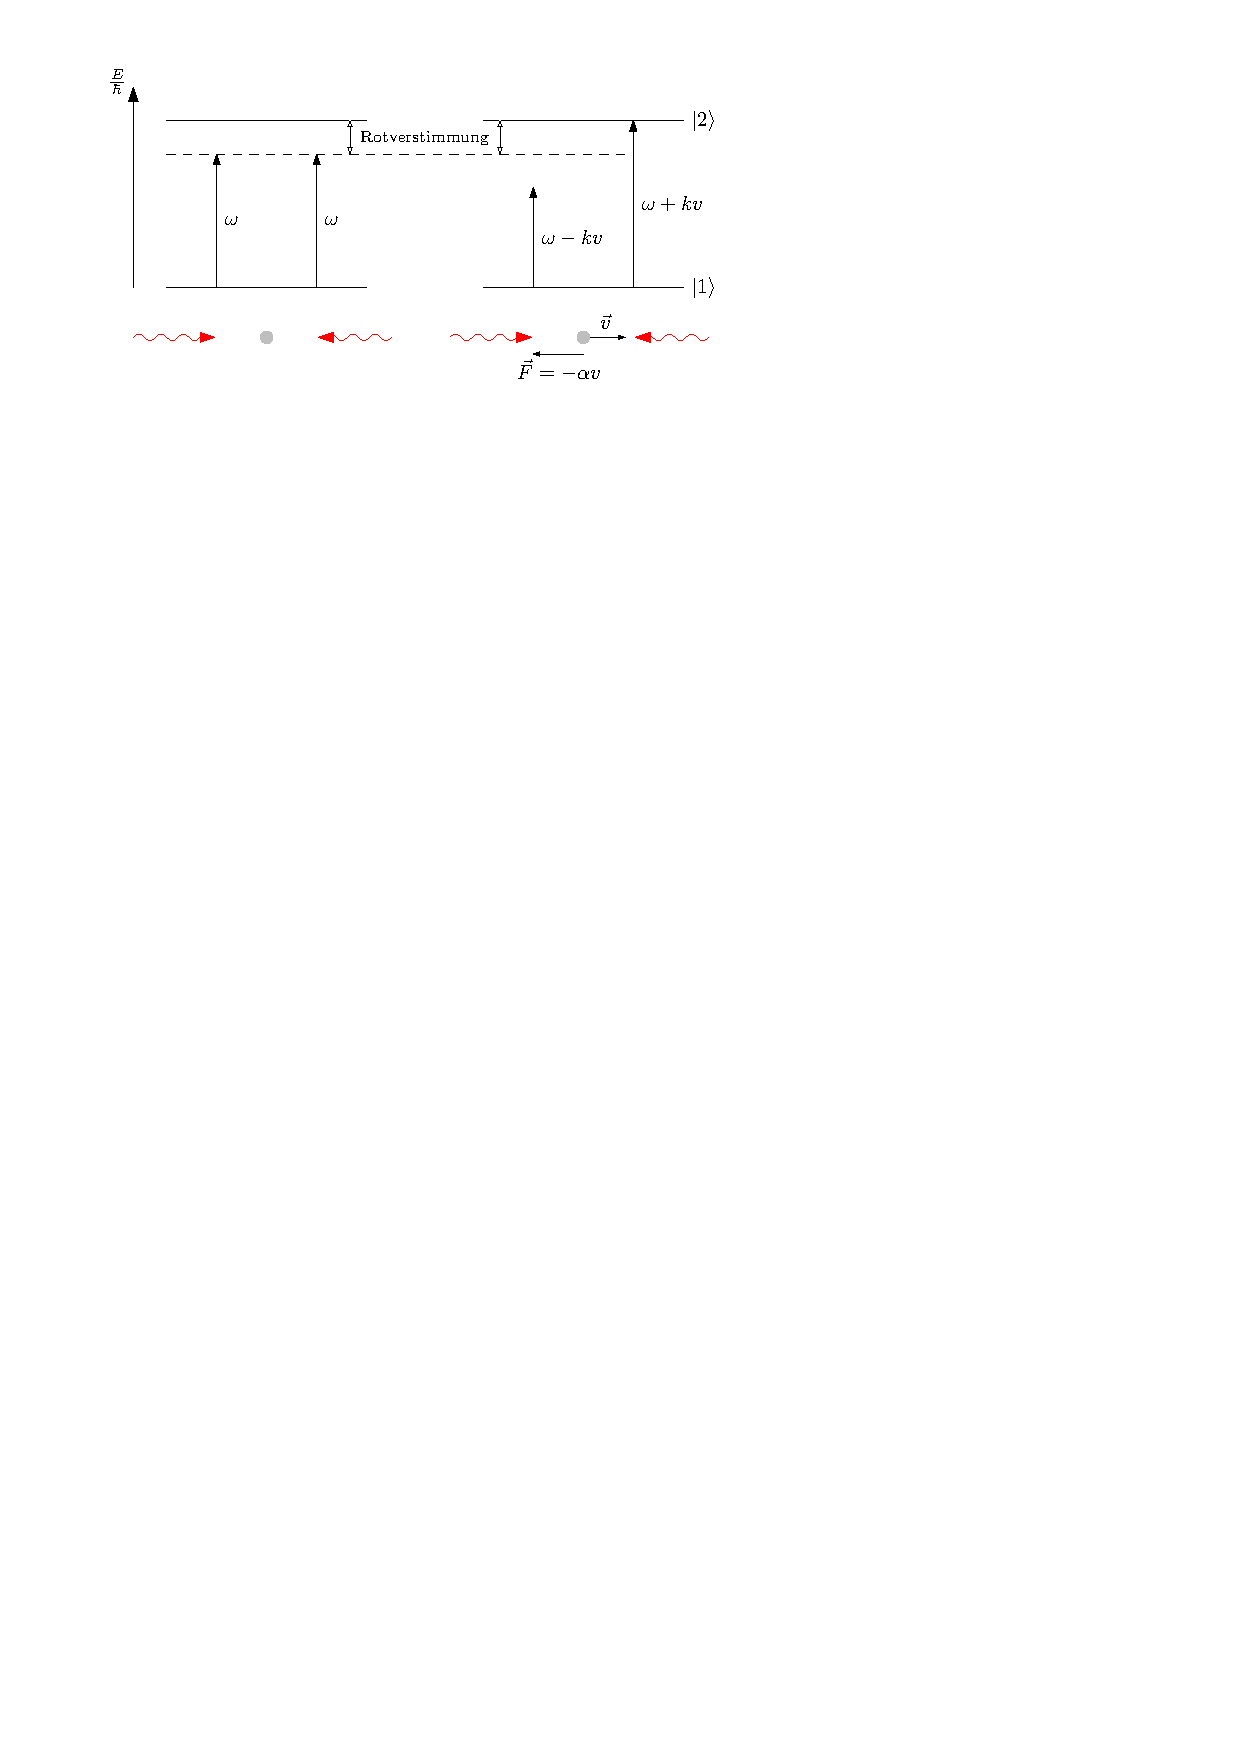
\includegraphics[width=.8\textwidth]{./figures/theory/melasse}
	\caption{Optische Melasse. Links: Kraftwirkung auf ein ruhendes Atom. Rechts: der Bewegung eines Atoms entgegengesetzte Kraft}
\end{figure}
Werden nun Laser auf drei zueinander senkrechten Achsen genutzt, welche so justiert werden, dass ihre Rückreflexion mit dem einfallenden Strahl überlagern, werden Atome im Kreuzungspunkt der Lichtstrahlen gekühlt, egal in welche Richtung sie sich bewegen.
Die entstehende Ansammlung kalter Atome wird als optische Melasse bezeichnet.

\subsection{Fangen von Atomen}

Um die gekühlten Atome, die sich zwar mit geringerer Geschwindigkeit aber weiterhin frei bewegen, an einem bestimmten Punkt zu konzentrieren wird der Zeeman-Effekt genutzt.
Dieser bewirkt eine Aufspaltung der atomaren Niveaus in drei Zustände mit $m_\mathrm{J} = 0, \pm1$, deren Energieverschiebung vom Zustand mit $m_\mathrm{J}=0$, was dem ursprünglichen Niveau entspricht, von der Stärke des Magnetfeldes abhängt.
Übergänge in diese Zustände können durch links- bzw. rechtszirkular polarisiertes Licht gezielt ausgewählt werden.

Für das Magnetfeld wird ein Spulenaufbau in Anti-Helmholtz-Konfiguration verwendet, der ein linear ansteigendes Magnetfeld in alle Richtungen ermöglicht.
Im Zentrum des Aufbaus verschwindet das Magnetfeld, hier werden die Atome gefangen.
Damit diese die Falle nicht verlassen werden aus entgegengesetzten Richtungen jeweils ein linkszirkular und ein rechtszirkular polarisierter Laser eingestrahlt, der entsprechend mit den aufgespaltenen Energieniveaus interagiert, siehe Abbildung \ref{fig:magnetfeld}.
\begin{figure}[h]
	\centering
	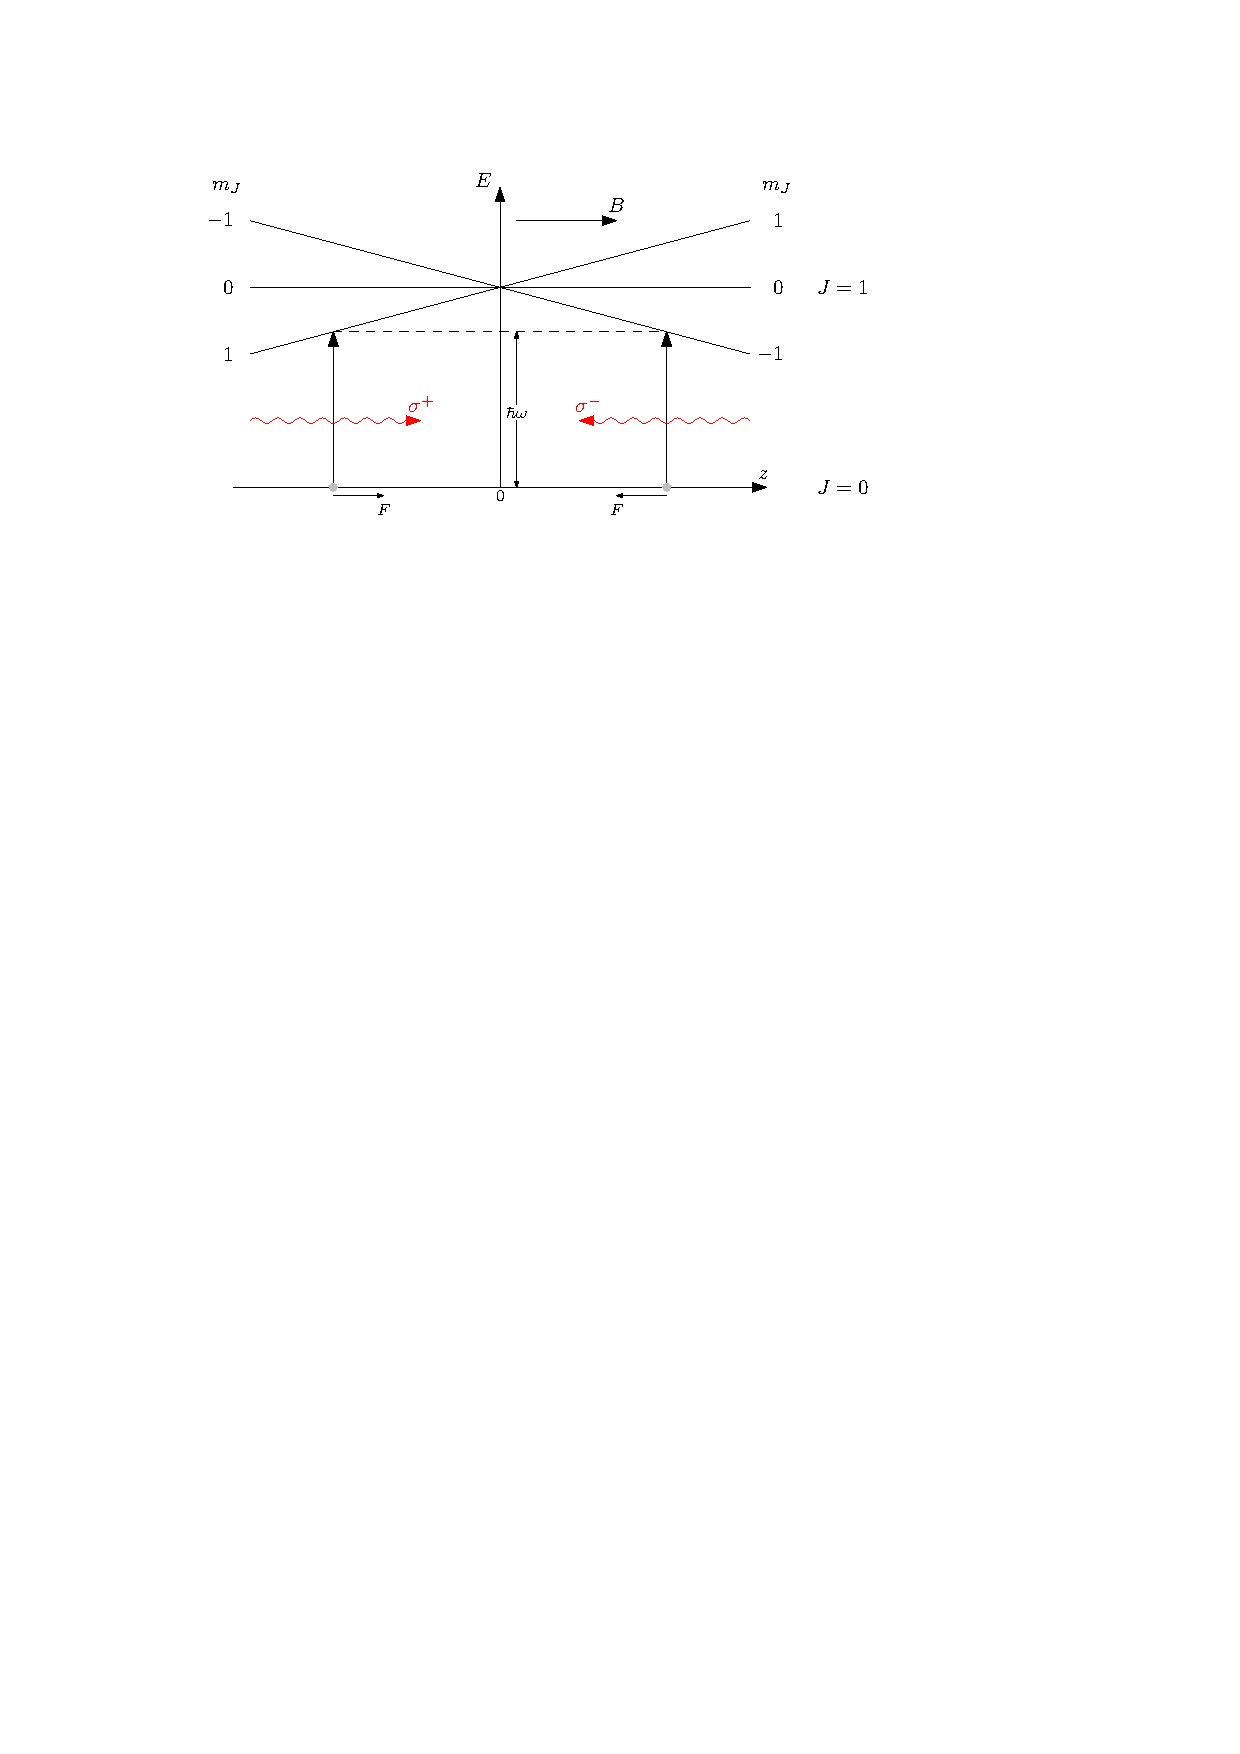
\includegraphics[width=.8\textwidth]{./figures/theory/mot.pdf}
	\caption{Nutzung des Zeeman-Effekts, um eine ortsabhängige Kraft auf die zu fangenden Teilchen auszuüben.\korr{Bild ändern, Beschriftungen vergrößern, Indizes aufrecht}}
	\label{fig:magnetfeld}
\end{figure}
Für ein nach links ausgelenktes Atom, d.h. im Bereich der Magnetfeldstärke $B<0$ liegt der Zustand mit $m_\mathrm{J}=+1$ unter dem nicht aufgespaltenen Energieniveau, so dass ein diesem Energieniveau gegenüber rotverstimmter Laser mit $\sigma^+$ Polarisation mit dem $m_\mathrm{J}=+1$ Zustand wechselwirkt und eine Kraft Richtung Zentrum der Falle auf das Atom ausübt.
Der analoge Fall gilt für ein nach rechts ausgelenktes Atom im Bereich von $B>0$, wo der von rechts eingestrahlte Laser mit $\sigma^-$ Polarisation mit dem $m_\mathrm{J}=-1$ Zustand wechselwirkt, der ebenfalls unterhalb des ursprünglichen Energieniveaus liegt.
Somit erhält man durch die gezielte Einstrahlung von polarisiertem Licht, welches entsprechend dem Magnetfeld polarisiert sein muss, eine ortsabhängige Kraft auf die Atome, die sie in das Zentrum der Falle drückt und somit ein Auseinanderlaufen der gekühlten Atome verhindert.

\section{Aufbau der MOT}

\subsection{Einstellung der Laserfrequenzen}

Zunächst wurden sowohl der Pump- als auch der Kühllaser auf die richtigen Frequenzen eingestellt.
Hierzu ist es wichtig, in den auf dem Oszilloskop beobachtbaren Spektren die richtigen Übergänge im Rubidium zu identifizieren, auf die die Laser eingestellt werden sollen.
Als Hilfe dienten die dargestellten Spektren in \cite{anleitung} für das \isotope[85]{Ru} Isotop.
Der Kühllaser wurde auf den Übergang $F=3 \rightarrow F\prime=4$ eingestellt, indem durch Änderung der Scanamplitude und des Scanoffsets das in der Polarisationspsketroskopie beobachtete Fehlersignal einen Nulldurchgang bei einer leichten Rotverschiebung gegenüber des gewünschten Rubidiumübergangs zeigt.
Durch fixieren dieses Signals mit dem Lock-Schalter an der Lockbox wird die Rückkopplungsschleife betrieben, die das Gitter am Diodenlaser ansteuert und damit die Frequenz reguliert.

Der Pumplaser wurde auf die gleiche Weise auf den $F=2 \rightarrow F\prime=3$ Übergang eingestellt, jedoch kann dieser Laser nicht über eine Rückkopplungsschleife auf eine Frequenz fixiert werden.
Da dieses Signal jedoch nicht mit der gleichen Genauigkeit wie beim Kühllaser eingestellt werden muss, ist ein Betrieb der Falle trotzdem möglich.

\subsection{Justage der Laser an der Vakuumkammer}

Mit einem Leistungsmessgerät wurde zunächst überpüft, ob genügend Licht aus der optischen Faser austritt, wobei eine Leistung von \SI{14,5}{mW} festgestellt werden konnte.
Durch zwei Strahlteiler wird das Laserlicht in drei Strahlen geteilt, die jeweils senkrecht zueinander stehen und die Vakuumkammer durchlaufen, bevor sie von einem Spiegel in sich selbst reflektiert werden, so dass insgesamt sechs Strahlen die Kammer auf drei Achsen passieren.
Zwei der Strahlen verlaufen in der horizontalen Ebene, einer entlang der vertikalen Achse.
Durch $\lambda/2$-PLatten kann die Leistung der einzelnen Teilstrahlen individuell eingestellt werden, wobei alle Strahlen ungefähr die gleiche Leistung haben sollten.
Für den vertikalen Strahl wurde eine Leistung vo \SI{3,0}{mW} eingestellt, für die beiden horizontalen \SI{3,0}{mW} bzw. \SI{3,2}{mW}.
Da diese Leistungen sich nicht zu den ursprünglich zur Verfügung stehenden \SI{14,5}{mW} addieren, kann festgestellt werden, dass in dem Aufbau eine Lichtleistung von ca. \SI{5,3}{mW} verloren geht.

Im Anschluss wurden die Aufbauten, d.h. die Spiegel und Einstellung der $\lambda/4$ Platten optimiert, so dass sich auf den drei Achsen sowohl einfallender als auch reflektierter Laserstrahl überlagern und sich die Strahlen im Zentrum der Vakuumkammer kreuzen.
Nach Einschalten des Magnetfeldes konnte mit der CCD-Kamera bereits eine Fluoreszenz und eine kleine Wolke gefangener Rubidiumatome erkennen.

\subsection{Optimierung der gefundenen Einstellungen}

Während eine Änderung der Rotverschiebung des Kühllasers nur eine geringe Auswirkung auf die Größe und Intensität der beobachteten Atome zeigte, konnte vor allem durch eine Feinjustage der Frequenz des Pumplasers die Falle optimiert werden.
Ein zusätzliches konstantes Magnetfeld verschlechterte das beobachtete Bild, so dass diese Möglichkeit zur Optimierung nicht genutzt wurde und im Folgenden nur die Frequenz des Pumplasers geändert wurde.
Nach Anbringen eines Leistungsmessgeräts zur Bestimmung der Fluoreszenzleistung der Falle konnte auch quantitativ eine Optimierung vorgenommen werden.
So konnte eine Leistung von \SI{114}{nW} erreicht werden, wobei dieser Wert aufgrund von Temperaturschwankungen im Raum und daher Änderungen der Laserfrequenz mit der Zeit eine leichte Veränderung erfuhr.
Nachdem sich näherungsweise ein thermisches Gleichgewicht eingestellt hatte, war diese Veränderung jedoch sehr gering, so dass die folgenden Messungen durchgeführt werden konnten, wobei gegebenenfalls zwischen zwei Messungen eine Nachjustierung erfolgte.

\section{Charakterisierung der MOT}
\label{sec:charakterisierung_mot}
Nachdem die MOT aufgebaut und auf möglichst hohe Fluoreszenz optimiert wurde, kann im Folgenden die Charakterisierung einiger Eigenschaften der Falle durchgeführt werden.

\subsection{Atomzahl in der MOT}
Im Folgenden soll die Anzahl der gefangenen Atome in der MOT bestimmt werden.
Dazu muss zunächst der Fluoreszenzleistung der gefangenen Atome und der Strahlradius des Lasers bestimmt werden.

\subsubsection{Bestimmung der Fluoreszenz der MOT}
Zur Bestimmung der Fluoreszenz der MOT wird die leuchtende Atomwolke mithilfe einer Linse auf ein Leistungsmessgerät abgebildet.
Dabei gilt es zu beachten, dass die so gemessene Leistung auch die Fluoreszenz von ungefangenen Atomen beinhaltet.
Daher wird nach jeder Messung das Magnetfeld der Falle deaktiviert um eine Hintergrundmessung durchzuführen und der so gemessene Hintergrund kann vom Fluoreszenzsignal abgezogen werden.
Somit wird die Fluoreszenzleistung, die die Atomwolke in dem von der Linse aufgespannten Raumwinkel emittiert, zu
\begin{align*}
	P_\mathrm{Linse} = \SI{114 +- 5}{nW}
\end{align*}
bestimmt.
Um die Fluoreszenzleistung zu erhalten, die im gesamten Raumwinkel von~$4\pi$ emittiert wird, kann
\begin{align*}
	P_\mathrm{tot} = P_\mathrm{Linse} \cdot \frac{A_\mathrm{tot}}{A_\mathrm{Linse}}
\end{align*}
genutzt werden.
Dabei beschreibt $A_\mathrm{Linse}$ die Fläche der Linse und $A_\mathrm{tot}$ die Oberfläche der Kugel mit einem Radius $R$, der dem Abstand der MOT zur Linse entspricht.
Somit erhält man
\begin{align*}
	P_\mathrm{tot} = P_\mathrm{Linse} \cdot \frac{4 \pi R^2}{\frac{1}{4} \pi d_\mathrm{Linse}^2} = P_\mathrm{Linse} \cdot \frac{16 R^2}{d_\mathrm{Linse}^2}
\end{align*}
und mit den gemessenen Werten für den Linsendurchmesser
\begin{align*}
	d_\mathrm{Linse} = \SI{2.5 +- 0.1}{cm} \, \text{,}
\end{align*}
sowie dem Abstand~$R$ zwischen MOT und Linse
\begin{align*}
	R = \SI{10.3 +- 0.2}{cm}
\end{align*}
kann die gesamte Leistung berechnet werden.
Diese ergibt sich zu
\begin{align*}
	P_\mathrm{tot} = \SI{30.9 +- 3.1}{\micro\watt} \, \text{,}
\end{align*}
wobei der Fehler durch \textsc{Gauß}sche Fehlerfortpflanzung gemäß
\begin{align*}
	\Delta P_\mathrm{tot} = \frac{16}{d_\mathrm{Linse}^3} \sqrt{4 R^2 P_\mathrm{Linse}^2 d_\mathrm{Linse}^2 \Delta R^2 + R^4 \left( d_\mathrm{Linse}^2 \Delta P_\mathrm{Linse}^2 + 4 P_\mathrm{Linse}^2 \Delta d_\mathrm{Linse}^2 \right)}
\end{align*}
berechnet wurde.


\subsubsection{Bestimmung des Strahlradius}
Anschließend muss eine Bestimmung des Radius des Laserstrahls durchgeführt werden.
Dazu wird das Leistungsmessgerät in den Strahlengang gestellt und der Laser wird seitlich durch eine Messerklinge blockiert.
Durch eine Messung der Leistung des teilweise blockierten Laserstrahls in Abhängigkeit der Position der Klinge kann der Strahlradius bestimmt werden.
Dazu wird angenommen, dass der Laserstrahl durch einen \textsc{Gauß}-Strahl beschrieben werden kann, weshalb die Intensität des Strahls in der transversalen Ebene durch
\begin{align*}
	I(x, y) = \frac{2 P_0}{\pi w^2} \exp\left(-\frac{2 (x^2 + y^2)}{w^2} \right)
\end{align*}
mit der Gesamtleistung des Strahls~$P_0$ und dem Strahlradius~$w$, das ist die Entfernung zum Strahlmittelpunkt bei dem die Intensität auf $\sfrac{1}{e^2}$ abgefallen ist, gegeben ist.
Durch Integration kann nun die Leistung des teilweise blockierten Strahls bestimmt werden
\begin{align}
	P(x) &= \int_{x}^{\infty} \mathrm{d}x^\prime \int_{-\infty}^{\infty} \mathrm{d}y^\prime \, I(x^\prime, y^\prime) \\
	     &= \frac{P_0}{2} \left[ 1 - \erf\left( \frac{\sqrt{2} x}{w}\right) \right] \, \text{,}
	\label{eq:erf_fit}
\end{align}
wobei $x$ den von der Klinge blockierten Teil des Strahls beschreibt.

\begin{figure}
	\centering
	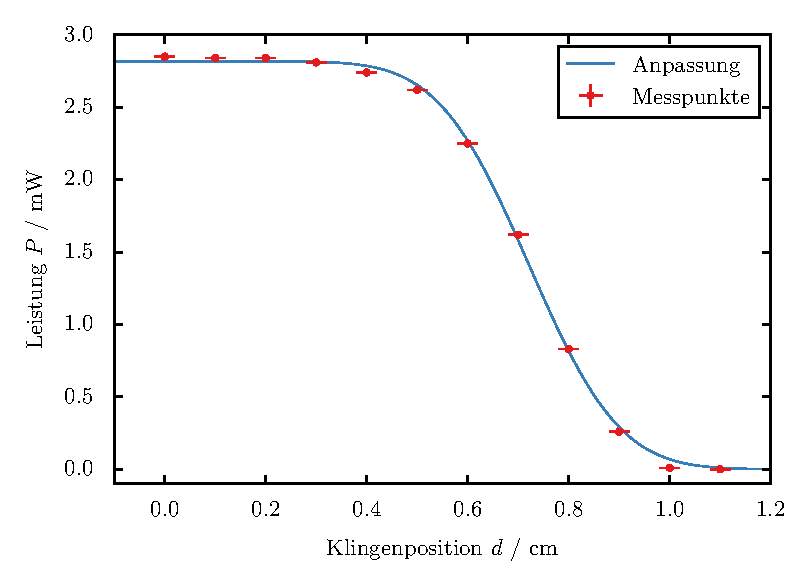
\includegraphics{./figures/beam_radius_fit.pdf}
	\caption{Anpassung einer Funktion gemäß der Hypothese in Gleichung~\eqref{eq:erf_fit} an die transmittierten Leistungen~$P$ nach der Blockierung des Strahlengangs mit einer Klinge an der Position~$x$. Der Fehler der Leistung~$\Delta P$ liegt in der Größenordnung der Markierung.}
	\label{fig:beam_radius}
	
	\vspace{1cm}
	
	\begin{tabular}{S[table-format=1.1]S[table-format=1.1]S[table-format=1.2]S[table-format=1.2]}
\toprule
{$x$ / \si{mm}} & {$\Delta x$ / \si{mm}} & {$P$ / \si{mW}} & {$\Delta P$ / \si{mW}} \\
\midrule
            0.0 &                    0.2 &            2.85 &                   0.02 \\
            1.0 &                    0.2 &            2.84 &                   0.02 \\
            2.0 &                    0.2 &            2.84 &                   0.02 \\
            3.0 &                    0.2 &            2.81 &                   0.02 \\
            4.0 &                    0.2 &            2.74 &                   0.02 \\
            5.0 &                    0.2 &            2.62 &                   0.02 \\
            6.0 &                    0.2 &            2.25 &                   0.02 \\
            7.0 &                    0.2 &            1.62 &                   0.02 \\
            8.0 &                    0.2 &            0.83 &                   0.02 \\
            9.0 &                    0.2 &            0.26 &                   0.02 \\
           10.0 &                    0.2 &            0.01 &                   0.02 \\
           11.0 &                    0.2 &            0.00 &                   0.02 \\
\bottomrule
\end{tabular}

	\captionof{table}{Transmittierte Leistung des Strahls~$P$ in Abhängigkeit der Klingenposition~$x$ zur Bestimmung des Strahlradius~$w$.}
	\label{tab:beam_radius}	
\end{figure}

Da in der Praxis keine relative Messung von Klingenposition~$x$ zum Strahlmittelpunkt durchgeführt werden kann, wird stattdessen eine Anpassung der um $\mu$ verschobenen Funktion $P(x-\mu)$ an die gemessenen Leistungen durchgeführt, um aus der Messung die Strahlleistung~$P_0$, den Strahlradius~$w$ und den Strahlmittelpunkt~$\mu$ zu extrahieren.
Die Anpassung einer solchen Kurve an die gemessenen Werte aus Tabelle~\ref{tab:beam_radius} 
führt zu den Anpassungsparametern:
\begin{align*}
	P_0 &= \SI{2.818 +- 0.017}{mW} \\
	w &= \SI{2.826 +- 0.089}{mm} \\
	\mu &= \SI{7.217 +- 0.033}{mm} \, \text{.}
\end{align*}
Die Messpunkte sowie die Anpassung wurden in Abbildung~\ref{fig:beam_radius} dargestellt.
Durch die Anpassung wurde demnach der Strahlradius~$w$ zu \SI{2.826 +- 0.089}{mm} bestimmt und kann folglich für die Auswertung verwendet werden.


\subsubsection{Bestimmung der Anzahl der gefangenen Atome}
\korr{TODO: Detuning fehlt}



\subsection{Größe der MOT}
Zur Bestimmung der Größe wird mit der CCD-Kamera ein Bild der in der Falle gefangenen Atome erstellt.
Um die Größe anzugeben, wurde im Anschluss bei gleicher Brennweite eine Millimeterskala im gleichen Abstand wie die Falle aufgenommen.
Dadurch konnte der Längenmaßstab der Aufnahmen zu~$\SI{1}{px}=\SI{0,0377}{mm}$ \korr{Fehler \& evtl.\ Bild von der Skala} bestimmt werden.
Entsprechend beträgt die Fläche eines Pixels dann~\SI{1.4213e-3}{mm^2} \korr{Fehler}.
Mit einem Bildbearbeitungsprogramm wurden in dem aufgenommenen Bild mehrere Strecken vermessen \korr{unklar}, da die beobachtete Atomwolke keiner einfachen geometrischen Figur ähnelt.
Die gemessenen Strecken wurden im Anschluss gemittelt und so ein Durchmesser von ungefähr \SI{1,47+-0,12}{mm} ermittelt werden \korr{Woher der Fehler}.
Durch eine Zählung der Pixel konnte weiterhin die Fläche zu \SI{1,16+-0,2}{mm^2} bestimmt werden.
Der Fehler wurde in diesem Fall abgeschätzt aufgrund von einer möglicherweise nicht idealen Auswahl des zu vermessenden Bereichs und entspricht einer Abweichung von~\num{162} Pixeln.
In Abbildung \ref{fig:mot_groesse} ist der untersuchte Bereich zur Bestimmung von Durchmesser und Fläche zu sehen.
\begin{figure}[h]
	\centering
	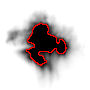
\includegraphics[width=.7\textwidth]{./figures/size_inverted.png}
	\caption{Zur Auswertung genutzter Bereich im mit der CCD-Kamera aufgenommenen Bild. Für eine bessere Druckqualität wurden die Farben invertiert.}
	\label{fig:mot_groesse}
\end{figure}

\subsection{Einfluss der $\lambda / 4$-Platten}
Im Folgenden soll der Einfluss der $\lambda / 4$-Platten auf die Population der Falle untersucht werden.
Dazu wird erneut die MOT durch eine Linse auf das Leistungsmessgerät abgebildet, um ein Fluoreszenzsignal zu messen.
Die im Aufbau auftretenden $\lambda / 4$-Verzögerungsplatten lassen sich in zwei Gruppen einteilen.
Diese sind die Platten für den in die Falle eingehenden Strahl und die für den reflektierten Strahl direkt am retroreflektierenden Spiegel.
Da da der Einfluss der einzelnen Platten für die jeweilige Fallenachse identisch ist, wird im Folgenden nur eine Achse detailliert untersucht.

\subsubsection{Verzögerungsplatte des eingehenden Strahls}
\label{sec:lambda_4_inc}
Zur Untersuchung des Einflusses der Verzögerungsplatte des eingehenden Strahls wird diese Schrittweise gedreht und sowohl der Stellungswinkel~$\varphi$ sowie die Fluoreszenzleistung~$P$ (mit subtrahiertem Untergrund) gemessen.
Dabei wird der Stellungswinkel schrittweise von \SI{0}{\degree} bis \SI{180}{\degree} in \SI{10}{\degree}-Schritten verstellt, bis ein gesamter Winkelbereich von \SI{180}{\degree} vermessen wurde.
Die somit gemessene Fluoreszenzleistung in Abhängigkeit des Drehwinkels der Platte für den eingehenden Strahl wurde in Abbildung \ref{fig:lambda_4_inc} aufgetragen.
Die gemessenen Werte wurden in Tabelle \ref{tab:lambda_4} zusammengefasst.
\begin{figure}[h]
	\centering
	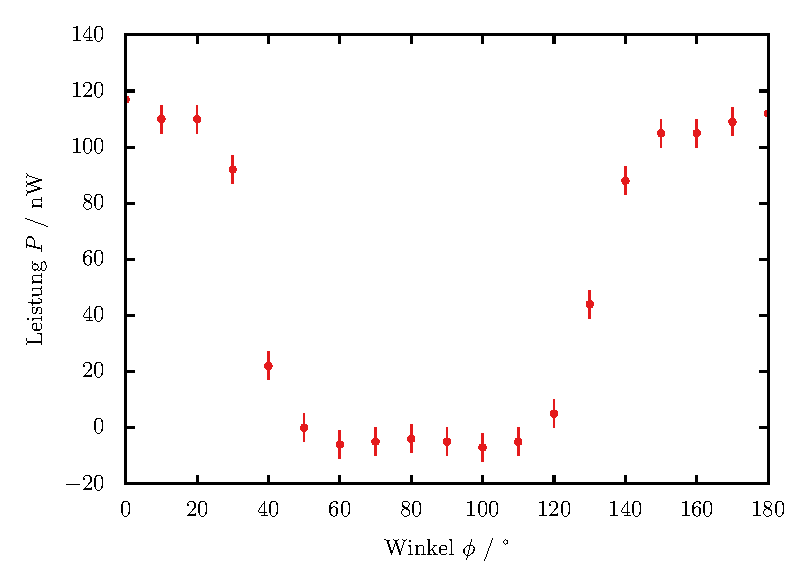
\includegraphics{./figures/lambda_4_in.pdf}
	\caption{Einfluss des Stellwinkels $\varphi$ der $\lambda / 4$-Platte des eingehenden Strahls auf die Fluoreszenz $P$ der MOT.}
	\label{fig:lambda_4_inc}
\end{figure}

Man sieht, dass die Stellung der $\lambda / 4$-Platte des eingehenden Strahls einen starken Einfluss auf die Fluoreszenzleistung zeigt.
Dies liegt daran, dass diese Platte den eintreffende linear-polarisierte Strahl in die für die Fallenoperation notwendige zirkulare Polarisation umwandelt.
Dazu muss die Achse der Verzögerungsplatte um $\pm\SI{45}{\degree}$ gegen die Polarisation des eintreffenden Strahls verkippt sein.
Darüber hinaus muss die richtige Zirkularpolarisation für diese Platte eingestellt werden, um die gemäß Abschnitt \korr{Theorie} erforderlichen Übergang zu treffen, der eine Operation der Falle ermöglicht.

In Abbildung \ref{fig:lambda_4_inc} sieht man, dass die Fluoreszenzleistung ein breites Minimum um einen Winkel der Verzögerungsplatte von \SI{80}{\degree} aufweist.
An dieser Stelle weist der Strahl gerade die falsche Zirkularpolarisation für das Fangen der Rubidiumatome auf.
Demnach sollte ein Drehen der Verzögerungsplatte um \SI{90}{\degree} nun die entgegengesetzte Zirkularpolarisation erzeugen und somit den Fallenbetrieb ermöglichen.
Dies entspricht dem breiten Maximum bei etwa \SI{170}{\degree}, bei dem der korrekte Übergang zum Fangen der Atome angeregt wird und somit den Fallenbetrieb ermöglicht.
Der auf der Verzögerungsplatte angegebene Optimalwert von \SI{172}{\degree} kann somit verifiziert werden.

Nach dem Abschluss dieser Messung werden die drei $\lambda / 4$-Platten für die eingehenden Strahlen per Hand auf das Maximum der Fluoreszenzleistung eingestellt.
Die Vergleich der Einstellung der Platten auf den verschiedenen Achsen~$\varphi$ mit den angegebenen Optimalwerten~$\varphi^\mathrm{opt}$ zeigt eine gute Übereinstimmung:
\begin{alignat*}{2}
\varphi_x &= \SI{180}{\degree} \qquad &&\varphi_x^\mathrm{opt} = \SI{172}{\degree}\\
\varphi_y &= \SI{214}{\degree} \qquad &&\varphi_y^\mathrm{opt} = \SI{224}{\degree}\\
\varphi_z &= \SI{80}{\degree} \qquad &&\varphi_z^\mathrm{opt} = \SI{80}{\degree} \, \text{.}
\end{alignat*}


\subsubsection{Verzögerungsplatte des reflektierten Strahls}
Letztlich soll der Einfluss der Verzögerungsplatte des reflektierten Strahls auf die Fluoreszenzleistung der MOT untersucht werden.
Dabei wird analog zu Abschnitt \ref{sec:lambda_4_inc} vorgegangen und die Fluoreszenzleistung~$P$ gegen den Winkel der Platte~$\varphi$ aufgetragen.
Die gemessenen Werte finden sich in Tabelle \ref{tab:lambda_4} und die Darstellung der Fluoreszenzleistung in Abbildung \ref{fig:lambda_4_out}.
\begin{figure}[h]
	\centering
	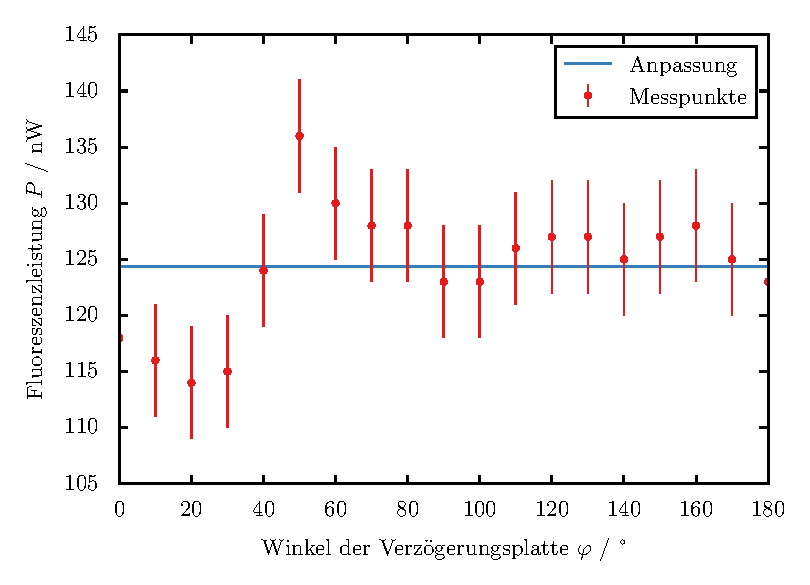
\includegraphics{./figures/lambda_4_out.pdf}
	\caption{Einfluss des Stellwinkels $\varphi$ der $\lambda / 4$-Platte des reflektierten Strahls auf die Fluoreszenz $P$ der MOT. Die Anpassung einer konstanten Funktion ergibt für die Fluoreszenzleistung $P_0 = \SI{124.4 +- 1.3}{nW}$.}
	\label{fig:lambda_4_out}
\end{figure}

Man sieht, dass die Fluoreszenzleistung kaum vom Winkel der Verzögerungsplatte abhängt.
Der Grund liegt darin, dass beim Eintreffen des zirkular-polarisierten Strahls aus dem Fallenzentrum auf die $\lambda / 4$-Platte dieser linear polarisiert wird.
Anschließend wird der linear-polarisierte Strahl am Spiegel reflektiert und trifft unter dem gleichen Winkel erneut auf die $\lambda / 4$-Platte und ist somit unabhängig von deren Stellwinkel.
Dies hat den Einfluss, dass die Helizität der Photonen umgekehrt wird und somit aus dem eingehenden Strahl mit $\sigma^\pm$-Polarisation ein rückläufiger Strahl mit $\sigma^\mp$-Polarisation entsteht.

Die Anpassung einer konstanten Funktion an die gemessene Fluoreszenzleistung ergibt
\begin{align*}
P_0 = \SI{124.4 +- 1.3}{nW}
\end{align*}
für die Fluoreszenzleistung der MOT.

\begin{table}
	\centering
	\begin{tabular}{S[table-format=3.0]S[table-format=3.0]S[table-format=3.0]}
\toprule
{$\varphi$ / \si{\degree}} & {$P_\mathrm{ein.}$ / \si{nW}} & {$P_\mathrm{ref.}$ / \si{nW}} \\
\midrule
                         0 &                           122 &                           118 \\
                        10 &                           115 &                           116 \\
                        20 &                           115 &                           114 \\
                        30 &                            97 &                           115 \\
                        40 &                            27 &                           124 \\
                        50 &                             5 &                           136 \\
                        60 &                            -1 &                           130 \\
                        70 &                             0 &                           128 \\
                        80 &                             1 &                           128 \\
                        90 &                             0 &                           123 \\
                       100 &                            -2 &                           123 \\
                       110 &                             0 &                           126 \\
                       120 &                            10 &                           127 \\
                       130 &                            49 &                           127 \\
                       140 &                            93 &                           125 \\
                       150 &                           110 &                           127 \\
                       160 &                           110 &                           128 \\
                       170 &                           114 &                           125 \\
                       180 &                           117 &                           123 \\
\bottomrule
\end{tabular}

	\caption{Gemessene Fluoreszenz der gefangenen Atome für verschiedene Stellungen der $\lambda / 4$-Platte des eingehenden Strahls~$P_\mathrm{ein.}$ und des reflektierten Strahls~$P_\mathrm{ref.}$. Auf die Fluoreszenzleistung wird ein Fehler von $\Delta P = \SI{5}{nW}$ angenommen.}
	\label{tab:lambda_4}
\end{table}


\subsection{Einfluss des Magnetfeldes}
Anschließend findet eine Messung der Fluoreszenzleistung der gefangenen Atome in Abhängigkeit des Stroms durch as Anti-Helmholtz-Spulenpaar statt.
Dieser Strom ist proportional zum Magnetfeldgradienten am Ort der Falle und hat somit einen Einfluss auf die Tiefe des Fallenpotentials.
Die gemessenen Werte der Fluoreszenzleistung~$P$ wurden in Abbildung~\ref{fig:magnetic_field} gegen den Spulenstrom~$I$ aufgetragen.
Darüber hinaus finden sich die gemessenen Werte in Tabelle~\ref{tab:magnetic_field}.
\begin{figure}[hp]
	\centering
	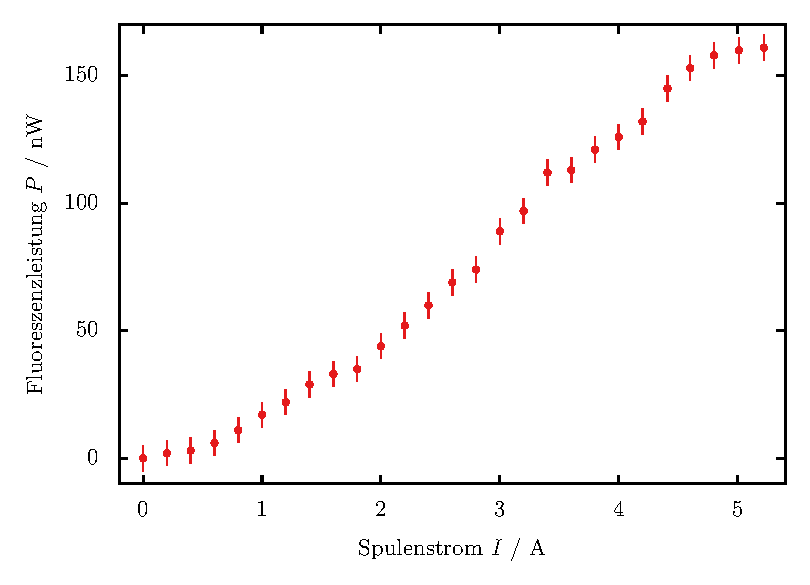
\includegraphics{./figures/magnetic_field.pdf}
	\caption{Einfluss des Spulenstroms des Anti-Helmholtz-Spulenpaares und somit des Magnetfeldgradienten im Zentrum der Falle auf die Fluoreszenzleistung der in der MOT gefangenen Atome.}
	\label{fig:magnetic_field}
	\vspace{1cm}
	\begin{minipage}[t]{0.3\textwidth}
		\centering
		\vspace*{-\dimexpr\baselineskip+\heavyrulewidth+\abovetopsep\relax}
		\begin{tabular}{S[table-format=1.2]S[table-format=3.0]}
\toprule
{Strom $I$ / \si{A}} & {Leistung $P$ / \si{nW}} \\
\midrule
                5.22 &                      161 \\
                5.01 &                      160 \\
                4.80 &                      158 \\
                4.60 &                      153 \\
                4.41 &                      145 \\
                4.20 &                      132 \\
                4.00 &                      126 \\
                3.80 &                      121 \\
                3.60 &                      113 \\
                3.40 &                      112 \\
                3.20 &                       97 \\
                3.00 &                       89 \\
                2.80 &                       74 \\
                2.60 &                       69 \\
\bottomrule
\end{tabular}

	\end{minipage} 
	\begin{minipage}[t]{0.3\textwidth}
		\centering
		\vspace*{-\dimexpr\baselineskip+\heavyrulewidth+\abovetopsep\relax}
		\begin{tabular}{S[table-format=1.2]S[table-format=3.0]}
\toprule
{Strom $I$ / \si{A}} & {Leistung $P$ / \si{nW}} \\
\midrule
                2.40 &                       60 \\
                2.20 &                       52 \\
                2.00 &                       44 \\
                1.80 &                       35 \\
                1.60 &                       33 \\
                1.40 &                       29 \\
                1.20 &                       22 \\
                1.00 &                       17 \\
                0.80 &                       11 \\
                0.60 &                        6 \\
                0.40 &                        3 \\
                0.20 &                        2 \\
                0.00 &                        0 \\
\bottomrule
\end{tabular}

	\end{minipage}
	\captionof{table}{Messwerte zur Bestimmung des Einflusses des Spulenstroms~$I$ mit einem Fehler von $\Delta I = \SI{0.01}{\ampere}$ auf die Fluoreszenzleistung der gefangenen Atome $P$ mit $\Delta P = \SI{5}{nW}$.}
	\label{tab:magnetic_field}
\end{figure}

Die Abbildung kann im wesentlichen in drei unterschiedliche Bereiche eingeteilt werden.
Zum einen ist dies der Bereich kleiner Ströme von \num{0} bis etwa \SI{1}{\ampere}, bei denen nur eine kleine Fluoreszenzleistung beobachtet werden kann, die nur langsam mit dem Spulenstrom ansteigt.
In diesem Strombereich ist der Potentialtopf zu klein um eine signifikante Anzahl von Atomen einzufangen.
Ab einem Strom von \SI{1}{\ampere} steigt die Fluoreszenzleistung stark mit dem Spulenstrom und die gefangenen Atome sind mithilfe einer Kamera klar zu erkennen.
An diesem Punkt können die Rubidiumatome effizient durch das Fallenpotential gefangen werden.
Übersteigt der Spulenstrom \SI{4.4}{\ampere} so stellt man fest, dass die Falle scheinbar in Sättigung übergeht.
\korr{Argument für die Sättigung}
Darüber hinaus finden sich einige Sprünge in den Messdaten deren Ursache bei dem Laser für das optische Pumpen der Rubidiumatome auf den Kühlübergang zu suchen sind.
Dieser kann aufgrund eines schlechten Fehlersignals nicht durch die Lockbox auf den Übergang festgestellt werden konnte und somit leichte Abweichungen während der Messung verursachte.


\subsection{Verhalten des Ladevorgangs}
Folglich soll das Verhalten des Ladevorgangs der Atomfalle untersucht werden.
Nun werden die gefangenen Atome durch eine Linse auf eine Photodiode abgebildet, welche eine zur Fluoreszenz der gefangenen Atome proportionale Spannung erzeugt, die folglich mit einem Oszilloskop gemessen werden kann.
Um einen Ladevorgang der Falle zu starten wird zunächst das Spulenstrom durch das Anti-Helmholtz-Spulenpaar deaktiviert sodass keine MOT mehr zu beobachten ist.
Danach wird das Magnetfeld reaktiviert und auf dem Oszilloskop kann ein exponentieller Anstieg der Fluoreszenz der gefangenen Atome beobachtet werden.
Dieser Anstieg verhält sich wie die Aufladung eines Kondensators und folglich wird die Anpassungshypothese
\begin{align}
	U(t) =  U_0 \left[ 1 - \exp\left( - \frac{t - t_0}{\tau} \right) \right] \cdot \Theta(t - t_0) + \mathrm{BG}
	\label{eq:loading_fit}
\end{align}
mit dem maximalen Fluoreszenzsignal~$U_0$ der Photodiode, der Zeitkonstante der Aufladung~$\tau$, der Beginn des Ladevorgangs~$t_0$, der Heaviside-Funktion~$\Theta$ und einem konstanten Untergrund~$\mathrm{BG}$.
In Abbildung \ref{fig:loading} wurde beispielhaft eine Anpassung an die Ladekurve durchgeführt.
Insgesamt wurden 11 Ladekurven zur Bestimmung der mittleren Zeitkonstante~$\bar{\tau}$ vermessen und die resultierenden Anpassungsparameter wurden in Tabelle~\ref{tab:loading_params} zusammengefasst.
\begin{figure}[htbp]
	\centering
	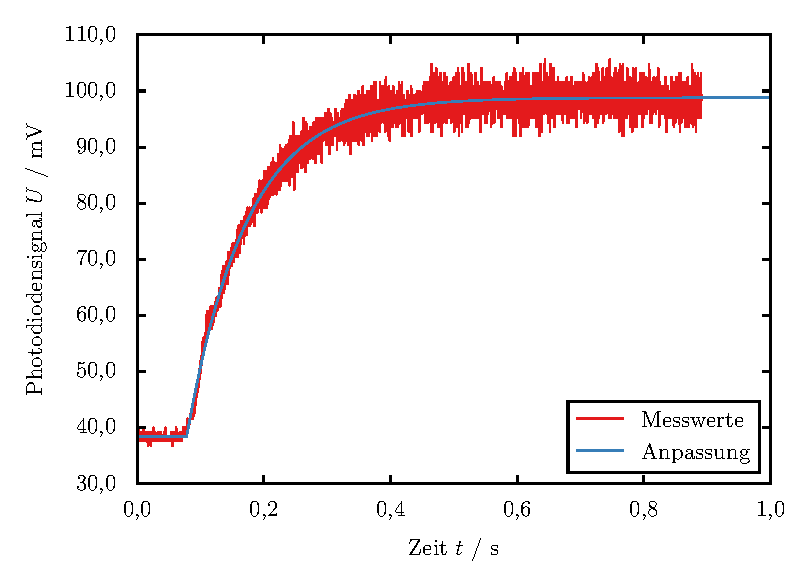
\includegraphics{./figures/loading/loading11.pdf}
	\caption{Anpassung einer Ladekurve gemäß der Anpassungshypothese in Gleichung \eqref{eq:loading_fit} an den zeitlichen Verlauf des Photodiodensignal~$U$ während des Ladevorgangs der MOT.}
	\label{fig:loading}
	
	\vspace{1cm}
	
	\resizebox{\textwidth}{!}{
		\begin{tabular}{S[table-format=2.2]S[table-format=1.2]S[table-format=3.2]S[table-format=1.2]S[table-format=3.2]S[table-format=1.2]S[table-format=2.2]S[table-format=1.2]}
\toprule
{$U_0$ / \si{mV}} & {$\Delta U_0$ / \si{mV}} & {$\tau$ / \si{ms}} & {$\Delta \tau$ / \si{ms}} & {$t_0$ / \si{ms}} & {$\Delta t_0$ / \si{ms}} & {$\mathrm{BG}$ / \si{mV}} & {$\Delta \mathrm{BG}$ / \si{mV}} \\
\midrule
            52.29 &                     0.22 &             105.09 &                      0.97 &             48.99 &                     0.71 &                     26.82 &                             0.20 \\
            52.52 &                     0.16 &             110.03 &                      0.94 &             80.53 &                     0.63 &                     27.07 &                             0.15 \\
            57.32 &                     0.17 &              97.52 &                      0.96 &            133.15 &                     0.62 &                     36.64 &                             0.14 \\
            55.88 &                     0.20 &              95.77 &                      0.95 &             86.37 &                     0.65 &                     37.41 &                             0.18 \\
            55.92 &                     0.22 &              99.23 &                      1.04 &            100.50 &                     0.72 &                     37.79 &                             0.20 \\
            50.23 &                     0.17 &              98.55 &                      1.17 &            141.01 &                     0.75 &                     38.57 &                             0.15 \\
            45.85 &                     0.27 &             103.74 &                      1.34 &             45.97 &                     0.99 &                     38.30 &                             0.26 \\
            35.51 &                     0.19 &             100.33 &                      1.64 &            109.21 &                     1.08 &                     35.35 &                             0.17 \\
            59.11 &                     0.16 &              96.21 &                      0.80 &             95.11 &                     0.53 &                     39.52 &                             0.14 \\
            56.95 &                     0.24 &              95.02 &                      0.95 &            126.57 &                     0.69 &                     38.20 &                             0.23 \\
            60.40 &                     0.19 &              94.33 &                      0.82 &             78.27 &                     0.57 &                     38.40 &                             0.17 \\
\bottomrule
\end{tabular}

	}
	\captionof{table}{Ergebnisse der Anpassungen gemäß Gleichung \eqref{eq:loading_fit} an die vermessenen Ladekurven der MOT.}
	\label{tab:loading_params}
\end{figure}

Schließlich kann aus den 11 vermessenen Ladekurven die mittlere Zeitkonstante~$\bar{\tau}$ des Aufladeprozesses bestimmt werden.
Diese beträgt
\begin{align*}
	\bar{\tau} = \SI{99.6 +- 4.9}{ms} \, \text{,}
\end{align*}
wobei der Fehler aus der Stichprobenvarianz abgeschätzt wird.






\subsection{Verstimmung der Laserfrequenzen}






\section{Fazit}


\FloatBarrier
% BIBLIOGRAPHIE
\vspace{\fill}
% Maximale Anzahl der Einträge in Klammer
% Zitieren mit \cite{lamport94}
\begin{thebibliography}{19}
\bibitem{anleitung}
	\emph{Advanced Laboratory Course (physics601): Description of Experiments}, BONN-AT-2016-01MP, Universität Bonn, Januar 2016
\end{thebibliography}

% APPENDIX
\begin{appendix}
\newpage
\section{Anhang}
\end{appendix}

\end{document}
